%% BEAMER THEME FLIP 2012: Main tex file for compiling
%$ Compile this file. 
%%
%% Copyright 2012 by Flip Tanedo
%% This file may be distributed and/or modified
%% 	1. under the LaTeX Project Public License and/or
%% 	2. under the GNU Public License.
%% 
%% If you e-mail Flip (pt267@cornell.edu) to say that you
%% like this style file, then it would make him smile.

%% Please see notes.txt for comments on Beamer Theme Flip 2013
%% By default, this template is meant to be run with XeLaTeX (for fonts)
%% To run in PDFLaTeX, remove fontspec and any font commands

%% Discussion of Beamer vs XeLaTeX vs LuaLaTeX
%% http://tex.stackexchange.com/questions/29497/xelatex-preventing-beamer-from-using-different-backgrounds



\documentclass[12 pt,xcolor={table}]{beamer}
\usetheme[
	bullet=circle,		% Other option: square
	bigpagenumber,		% circled page number on lower right
	topline=true,			% colored bar at the top of the frame 
	shadow=false,			% Shading for beamer blocks
	watermark=BG_lower,	% png file for the watermark
	]{Flip}


\newcommand{\titleimage}{title}			% Custom title 
\newcommand{\tanedo}{tanedolight}		% Custom author name
\newcommand{\CMSSMDM}{CMSSMDMlight.png}	% light background plot


%%%%%%%%%%
% FONTS %
%%%%%%%%%%

%% Default font: lmodern, doesn't require fontspec % solves some default warnings
\usepackage[T1]{fontenc}
\usepackage{lmodern}			
\usepackage{sfmath}		% Sans Serif Math, off by default


%% Protects fonts from Beamer screwing with them
%% http://tex.stackexchange.com/questions/10488/force-computer-modern-in-math-mode
\usefonttheme{professionalfonts}


%% XeLaTeX fonts: (comment out if you don't use XeLaTeX)

%% For advanced fonts: access local OS X fonts
\usepackage[no-math]{fontspec}		
%% This template uses typical OS X and Adobe fonts
\defaultfontfeatures{Mapping=tex-text}	% This seems to be important for mapping glyphs properly

\setmainfont{Gillius ADF Regular} % Beamer ignores "main font" in favor of sans font
\setsansfont{Gillius ADF Regular}	% This is the font that beamer will use by default
% \setmainfont{Gill Sans Light}		% Prettier, but harder to read

\setbeamerfont{title}{family=\fontspec{Gillius ADF Regular}}


\newcommand{\handwriting}{\fontspec{augie}} % From Emerald City, free font
% \newcommand{\handwriting}{}	% If you prefer no special handwriting font or don't have augie

%% Gill Sans doesn't look very nice when boldfaced
%% This is a hack to use Helvetica instead
%% Usage: \textbf{\forbold some stuff}
\newcommand{\forbold}{\fontspec{Gillius ADF Cond Bold}}
% \newcommand{\forbold}{} % if you want no special boldface



%%%%%%%%%%%%%%%%%%%%%%%%
% Usual LaTeX Packages %
%%%%%%%%%%%%%%%%%%%%%%%%


\usepackage{amsmath}
\usepackage{amsfonts}
\usepackage{amssymb}
\usepackage{graphicx}
\usepackage{mathrsfs} 			% For Weinberg-esque letters
\usepackage{cancel}				% For "SUSY-breaking" symbol
\usepackage{slashed}            % for slashed characters in math mode
\usepackage{bbm}                % for \mathbbm{1} (unit matrix)
\usepackage{amsthm}				% For theorem environment
\usepackage{multirow}			% For multi row cells in table
\usepackage{arydshln} 			% For dashed lines in arrays and tables
\usepackage{tikzfeynman}		% For Feynman diagrams
% \usepackage{subfig}           % for sub figures
% \usepackage{young}			% For Young Tableaux
% \usepackage{xspace}			% For spacing after commands
% \usepackage{wrapfig}			% for Text wrap around figures
% \usepackage{framed}


\graphicspath{{img/}}	% Put all images in this directory. Avoids clutter.

\usetikzlibrary{arrows,shapes}
\usetikzlibrary{fadings}
\usetikzlibrary{backgrounds}
\usetikzlibrary{mindmap,trees}	% For mind map
% http://www.texample.net/tikz/examples/computer-science-mindmap/


% SOME COMMANDS THAT I FIND HANDY
% \renewcommand{\tilde}{\widetilde} % dinky tildes look silly, dosn't work with fontspec
\newcommand{\comment}[1]{\textcolor{comment}{\footnotesize{#1}\normalsize}} % comment mild
\newcommand{\Comment}[1]{\textcolor{Comment}{\footnotesize{#1}\normalsize}} % comment bold
\newcommand{\COMMENT}[1]{\textcolor{COMMENT}{\footnotesize{#1}\normalsize}} % comment crazy bold
\newcommand{\Alert}[1]{\textcolor{Alert}{#1}} % louder alert
\newcommand{\ALERT}[1]{\textcolor{ALERT}{#1}} % loudest alert
%% "\alert" is already a beamer pre-defined



\author[Mandy Vogel\quad {mandy.vogel@googlemail.com}]{Mandy Vogel}
\title[Linear Models]{Linear Models Part II}
\institute{University Leipzig}
\date{\today}



\begin{document}

%%%%%%%%%%%%%%%%%%%%%%%%
% Additional  settings %
%%%%%%%%%%%%%%%%%%%%%%%%

%% To use external nodes;  http://www.texample.net/tikz/examples/beamer-arrows/
\tikzstyle{every picture}+=[remember picture]


\everymath{\displaystyle}

\tikzfading[name=fade inside,
            inner color=transparent!60,
            outer color=transparent!0]
%%%%%%%%%%%%%%%%%%%%%%%%
% Actual content below %
%%%%%%%%%%%%%%%%%%%%%%%%

%% It's much nicer to have all the content in a separate file


\AtBeginSection{
  \begin{frame}<beamer>[allowframebreaks,t]{Table of Contents}
    \tableofcontents[currentsection]
  \end{frame}}


\begin{frame}
\titlepage
\end{frame}

\begin{frame}{Overview}
  \tableofcontents
\end{frame}

\section{Recap}
\subsection{Simple Linear Model}

\begin{frame}
\frametitle{Simple Linear Model}

\tikzstyle{na} = [baseline=-.5ex]

% Below we mix an ordinary equation with TikZ nodes. Note that we have to
% adjust the baseline of the nodes to get proper alignment with the rest of
% the equation.
      $$y_i = \beta_0 + \beta_1\cdot x_i + \epsilon_i$$
\end{frame}



\begin{frame}
\frametitle{Simple Linear Model}

\tikzstyle{na} = [baseline=-.5ex]

% Below we mix an ordinary equation with TikZ nodes. Note that we have to
% adjust the baseline of the nodes to get proper alignment with the rest of
% the equation.
    \begin{equation*}
      \tikz[baseline]{
        \node[fill=blue!20,anchor=base] (t1){
          $y_i$ }; 
        } = 
      \tikz[baseline]{
        \node[anchor=base] (t2){
          $\beta_0 + \beta_1\cdot$ }; 
        }
      \tikz[baseline]{
        \node[fill=blue!20,anchor=base] (t3){
          $x_i$ }; 
        } +
      \tikz[baseline]{
        \node[anchor=base] (t4){
          $\epsilon_i$ }; 
        }
    \end{equation*}

\begin{itemize}[<+-| alert@+>]
    \item[]<1->\tikz \node [fill=blue!20,draw,circle] (n1) {}; the y variable is called response variable

    \item[]<2->\tikz \node [fill=blue!20,draw,circle] (n2) {}; the x variable is called the predictor variable, covariate, or regressor
        
\end{itemize}

\begin{tikzpicture}[overlay]
        \path[->]<1> (n1) edge [out= 180, in= 135] (t1);
        \path[->]<2> (n2) edge [out= 180, in= 135] (t3);
\end{tikzpicture}

\end{frame}


\begin{frame}
\frametitle{$y_i$ depends on}

\tikzstyle{na} = [baseline=-.5ex]

% Below we mix an ordinary equation with TikZ nodes. Note that we have to
% adjust the baseline of the nodes to get proper alignment with the rest of
% the equation.
    \begin{equation*}
      \tikz[baseline]{
        \node[anchor=base] (d1){
          $y_i$ }; 
        } = 
      \tikz[baseline]{
        \node[fill=blue!20,anchor=base] (u1){
          $\beta_0 + \beta_1\cdot$ }; 
        }
      \tikz[baseline]{
        \node[fill=green!20,anchor=base] (u2){
          $x_i$ }; 
        } + 
      \tikz[baseline]{
        \node[fill=red!20,anchor=base] (u3){
          $\epsilon_i$ }; 
        }
    \end{equation*}

\begin{itemize}[<+-| alert@+>]
    \item[]<1->\tikz \node [fill=green!20,draw,circle] (m1) {}; the values of $x_i$

    \item[]<2->\tikz \node [fill=blue!20,draw,circle] (m2) {}; the linear function $\beta_0 + \beta_1\cdot x$
    \item[]<3->\tikz \node [fill=red!20,draw,circle] (m3) {}; the value of the random variable $\epsilon_i \sim \mathcal{N}(0,\sigma)$ \tikz \node [coordinate] (m4) {};
        
\end{itemize}

\begin{tikzpicture}[overlay]
        \path[->]<1> (m1) edge [out= 180, in= 135] (u2);
        \path[->]<2> (m2) edge [out= 180, in= 135] (u1);
        \path[->]<3> (m4) edge [out= 0, in= 45] (u3.north east);
\end{tikzpicture}

\end{frame}
\begin{frame}[fragile]{In R this becomes}
\tikzstyle{na} = [baseline=-.5ex]
    \begin{equation*}
      \tikz[baseline]{
        \node[fill=green!20,anchor=base] (v1){
          $y_i$ }; 
        } = 
      \tikz[baseline]{
        \node[anchor=base] (v2){
          $\beta_0 + \beta_1\cdot$ }; 
        }
      \tikz[baseline]{
        \node[fill=blue!20,anchor=base] (v3){
          $x_i$ }; 
        } + 
      \tikz[baseline]{
        \node[anchor=base] (v4){
          $\epsilon_i$ }; 
        }
    \end{equation*}

    \begin{equation*}
      \text{\texttt{lm(}}
      \tikz[baseline]{
        \node[fill=green!20,anchor=base] (w1){
          $\text{\texttt{y}}$ }; 
        } \sim 
      \tikz[baseline]{
        \node[fill=blue!20,anchor=base] (w2){
          $\text{\texttt{x}}$ }; 
        } \text{\texttt{)}}
    \end{equation*}
\end{frame}

\begin{frame}{Remember}
  \begin{itemize}
  \item we had birth weight as response variable (\texttt{bweight})
  \item gestational age as a continous explanatory variable (\texttt{gestwks})
  \item hypertension status as discrete explanatory variable with two levels (yes and no) (\texttt{hyp})
  \end{itemize}
\end{frame}

\begin{frame}{Our Example I}
  \begin{itemize}
  \item one continous explanatory variable
  \item so we estimate one intercept ($\beta_0$ from above) and one slope ($\beta_1$ from above)
  \end{itemize}
\end{frame}

\begin{frame}[fragile]{Our Example I}\scriptsize
\begin{semiverbatim}
> m <- lm(abweight ~ gestwks, data=births)
> summary(m)

Call:
lm(formula = bweight ~ gestwks, data = births)

Residuals:
     Min       1Q   Median       3Q      Max 
-1698.40  -280.14    -3.64   287.61  1382.24 

Coefficients:
             Estimate Std. Error t value Pr(>|t|)    
(Intercept) -4489.140    340.899  -13.17   <2e-16 ***
gestwks       196.973      8.788   22.41   <2e-16 ***
---
Signif. codes:  0 ‘***’ 0.001 ‘**’ 0.01 ‘*’ 0.05 ‘.’ 0.1 ‘ ’ 1 

Residual standard error: 449.7 on 488 degrees of freedom
  (10 observations deleted due to missingness)
Multiple R-squared: 0.5073,	Adjusted R-squared: 0.5062 
F-statistic: 502.4 on 1 and 488 DF,  p-value: < 2.2e-16 
\end{semiverbatim}      
\end{frame}

\subsection{R-squared}
\begin{frame}{R-squared}
  \begin{itemize}
  \item the $R^2$ is the coefficient of determination
  \item in case of a simple linear regression $R^2=r^2$ where $r$ is the correlation coefficient
  \item more general: $$ R^2 = 1 - \frac{\text{RSS}}{\text{TSS}} = 1- \frac{\sum{(y_i - \hat{y}_i)^2}}{\sum(y_i - \overline{y})^2}= \frac{\sum{(\hat{y}_i - \overline{y})^2}}{\sum(y_i - \overline{y})^2}$$
  \item that means $R^2 \cdot 100$\% of the variation is explained by the model
  \item the \emph{adjusted} $R^2$ is adjusted for the number of coefficients (penalize models for having many covariates)
  \end{itemize}
  
\end{frame}

\begin{frame}[fragile]{Our Example I - visualization}
  \begin{itemize}
  \item we build first a scatterplot (\texttt{geom\_abline()})
  \item extract the coefficients from the model (\texttt{coef(m)})
\begin{verbatim}
> coef(m)
(Intercept)     gestwks 
 -4489.1398    196.9726 
\end{verbatim}
  \item using \texttt{geom\_abline()} which take the intercept and the slope as arguments
  \end{itemize}\footnotesize
\end{frame}


\subsection{Visualization}
\begin{frame}[fragile]{Our Example I - visualization}
\begin{semiverbatim}
> ggplot(births, aes(x = gestwks,y = bweight)) +
+     geom_point() +
+     geom_abline(intercept = coef(m)[1],
+                 slope = coef(m)[2])
Warnmeldung:
Removed 10 rows containing missing values (geom_point).  
\end{semiverbatim}      
\end{frame}



\begin{frame}[shrink=5]\frametitle{Our Example I - visualization}
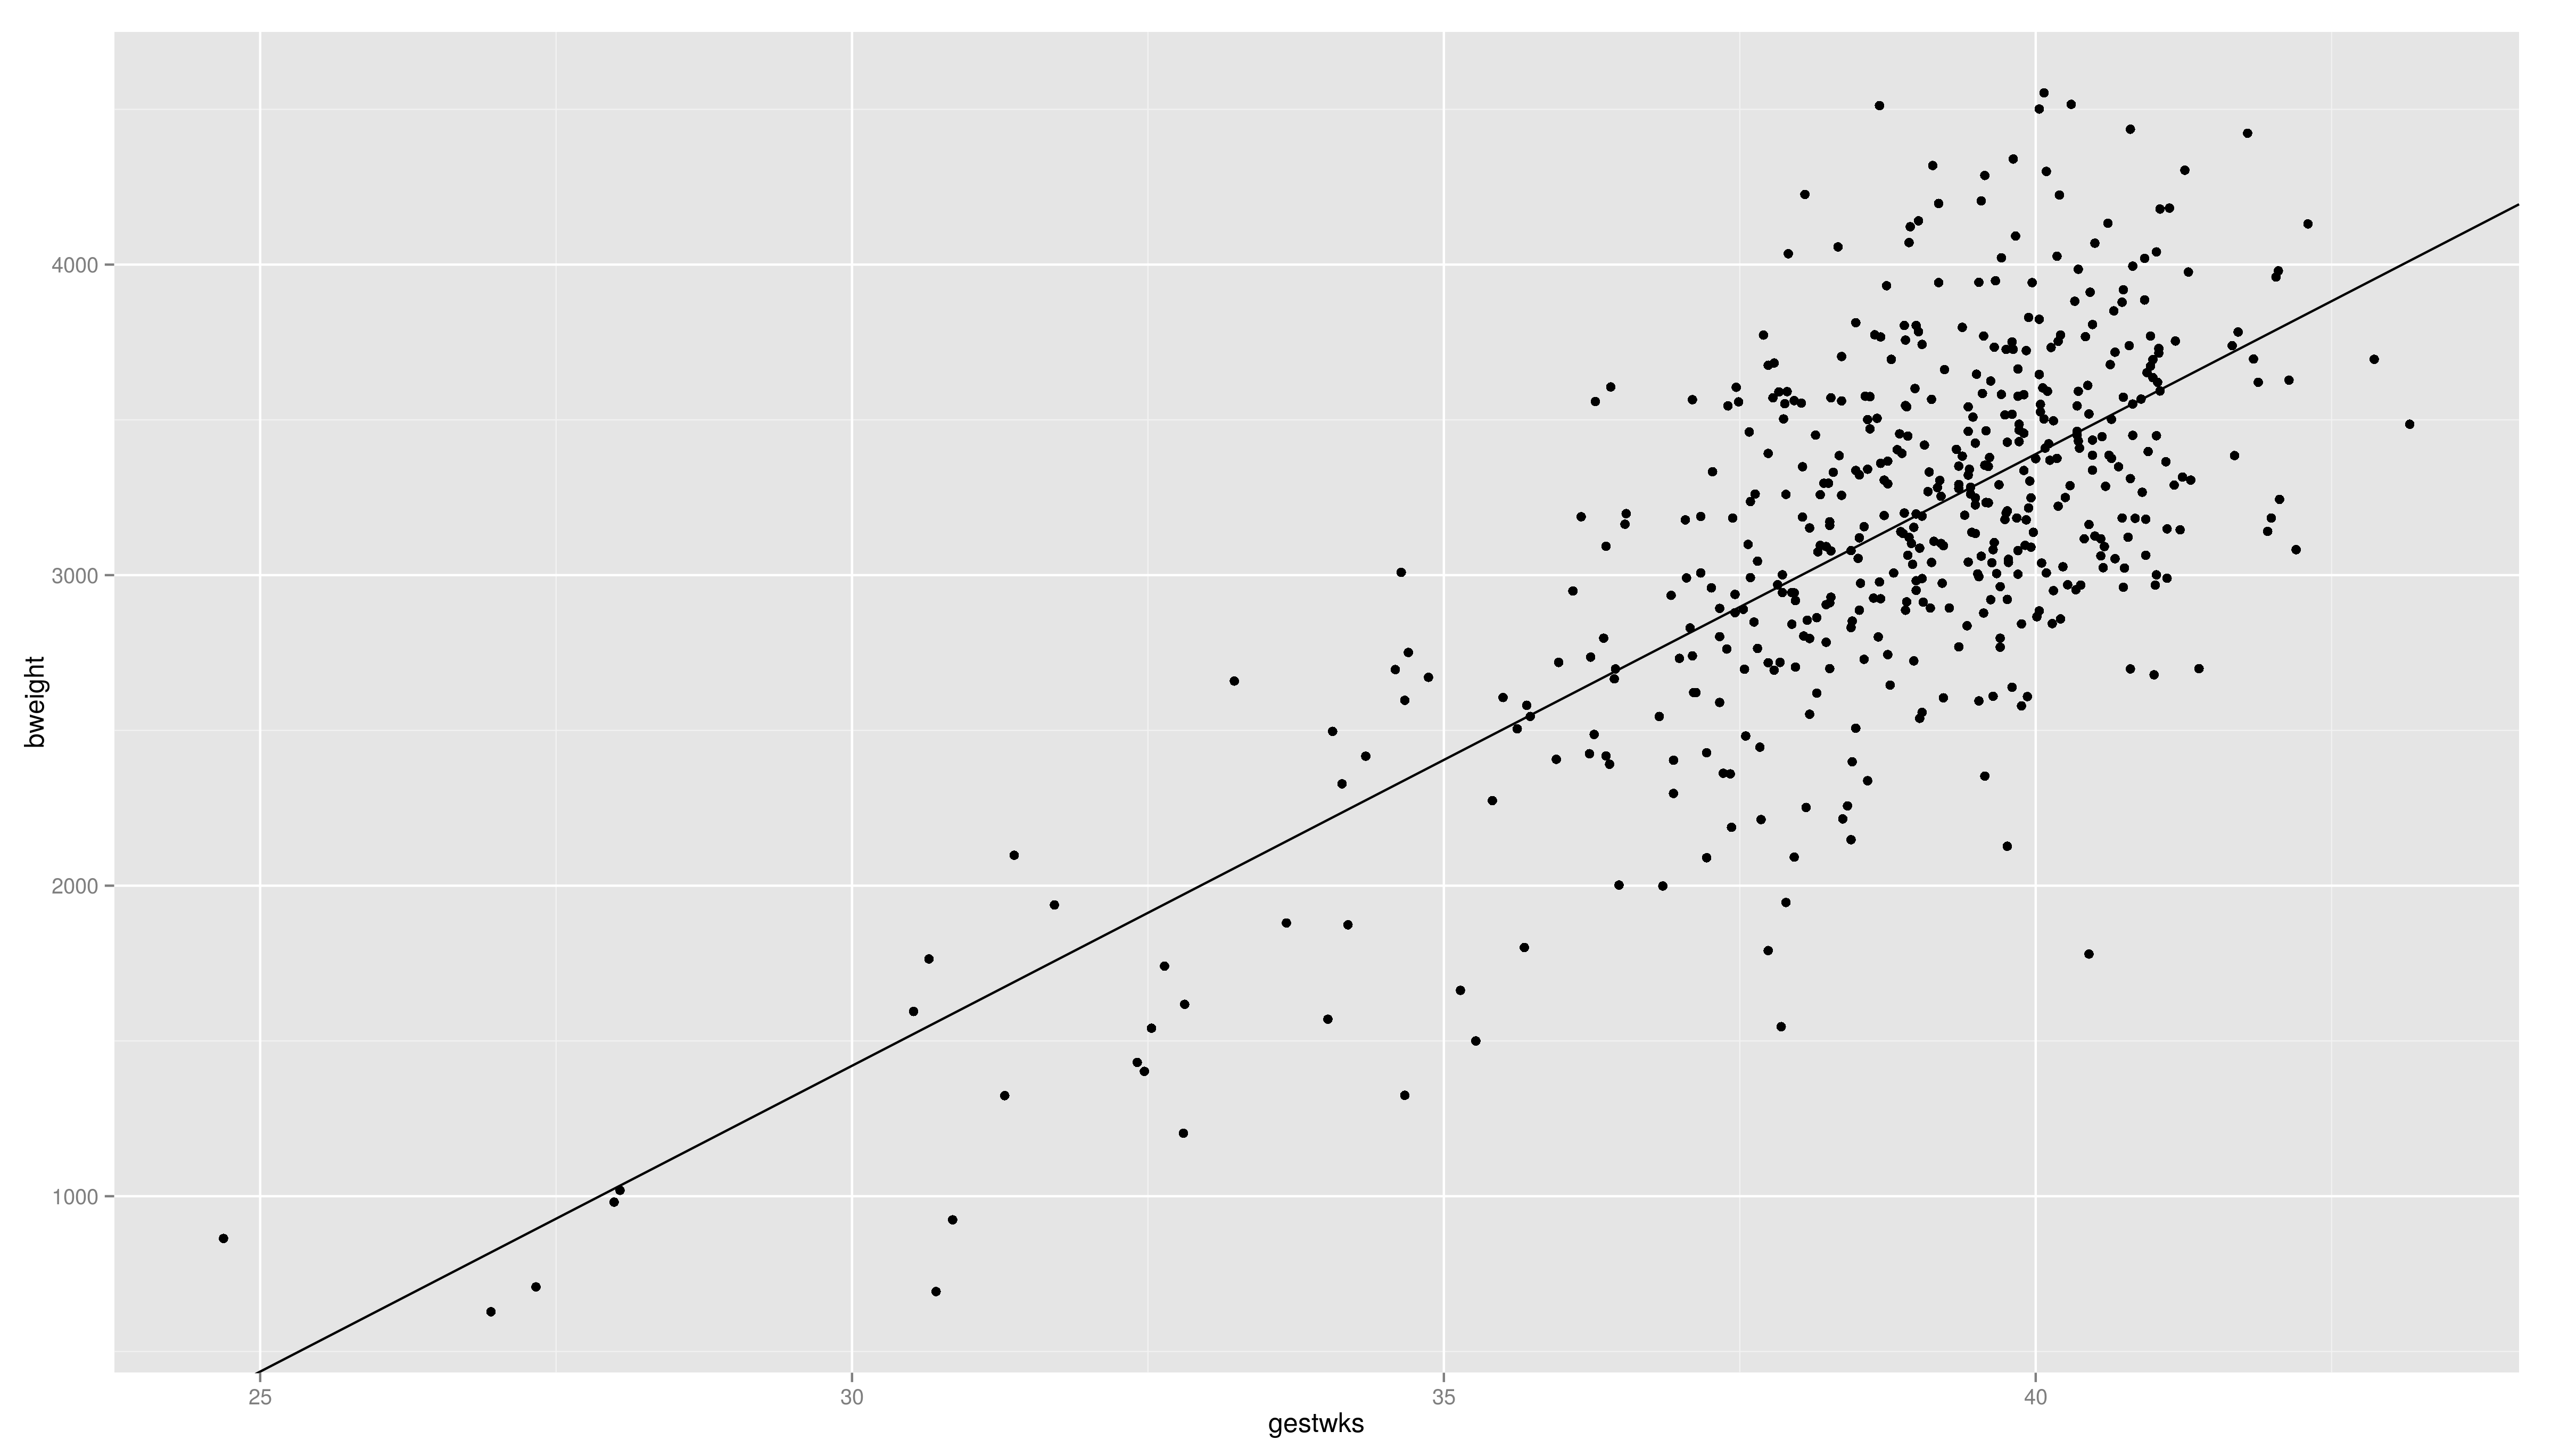
\includegraphics[height=7cm]{model1.png}

The effect of \texttt{gestwks} is the slope of the line 
\end{frame}


\begin{frame}{Our Example II}
  \begin{itemize}
  \item we add one discrete explanatory variable
  \item so we estimate two intercepts, one for each level of \texttt{hyp} 
  \item and one slope ($\beta_1$ from above)
  \end{itemize}
\end{frame}



\begin{frame}[fragile]{Our Example II}\scriptsize
\begin{semiverbatim}
> m <- lm(bweight ~ hyp + gestwks, data=births)
> summary(m)

Call:
lm(formula = bweight ~ hyp + gestwks, data = births)

Residuals:
     Min       1Q   Median       3Q      Max 
-1711.04  -283.13    -9.86   283.92  1361.22 

Coefficients:
             Estimate Std. Error t value Pr(>|t|)    
(Intercept) -4285.002    349.322 -12.267   <2e-16 ***
hyphyper     -143.675     58.820  -2.443   0.0149 *  
gestwks       192.238      8.956  21.465   <2e-16 ***
---
Signif. codes:  0 ‘***’ 0.001 ‘**’ 0.01 ‘*’ 0.05 ‘.’ 0.1 ‘ ’ 1

Residual standard error: 447.5 on 487 degrees of freedom
  (10 observations deleted due to missingness)
Multiple R-squared:  0.5132,	Adjusted R-squared:  0.5112 
F-statistic: 256.7 on 2 and 487 DF,  p-value: < 2.2e-16
\end{semiverbatim}
\end{frame}

\begin{frame}[shrink=5]\frametitle{Our Example II - visualization}
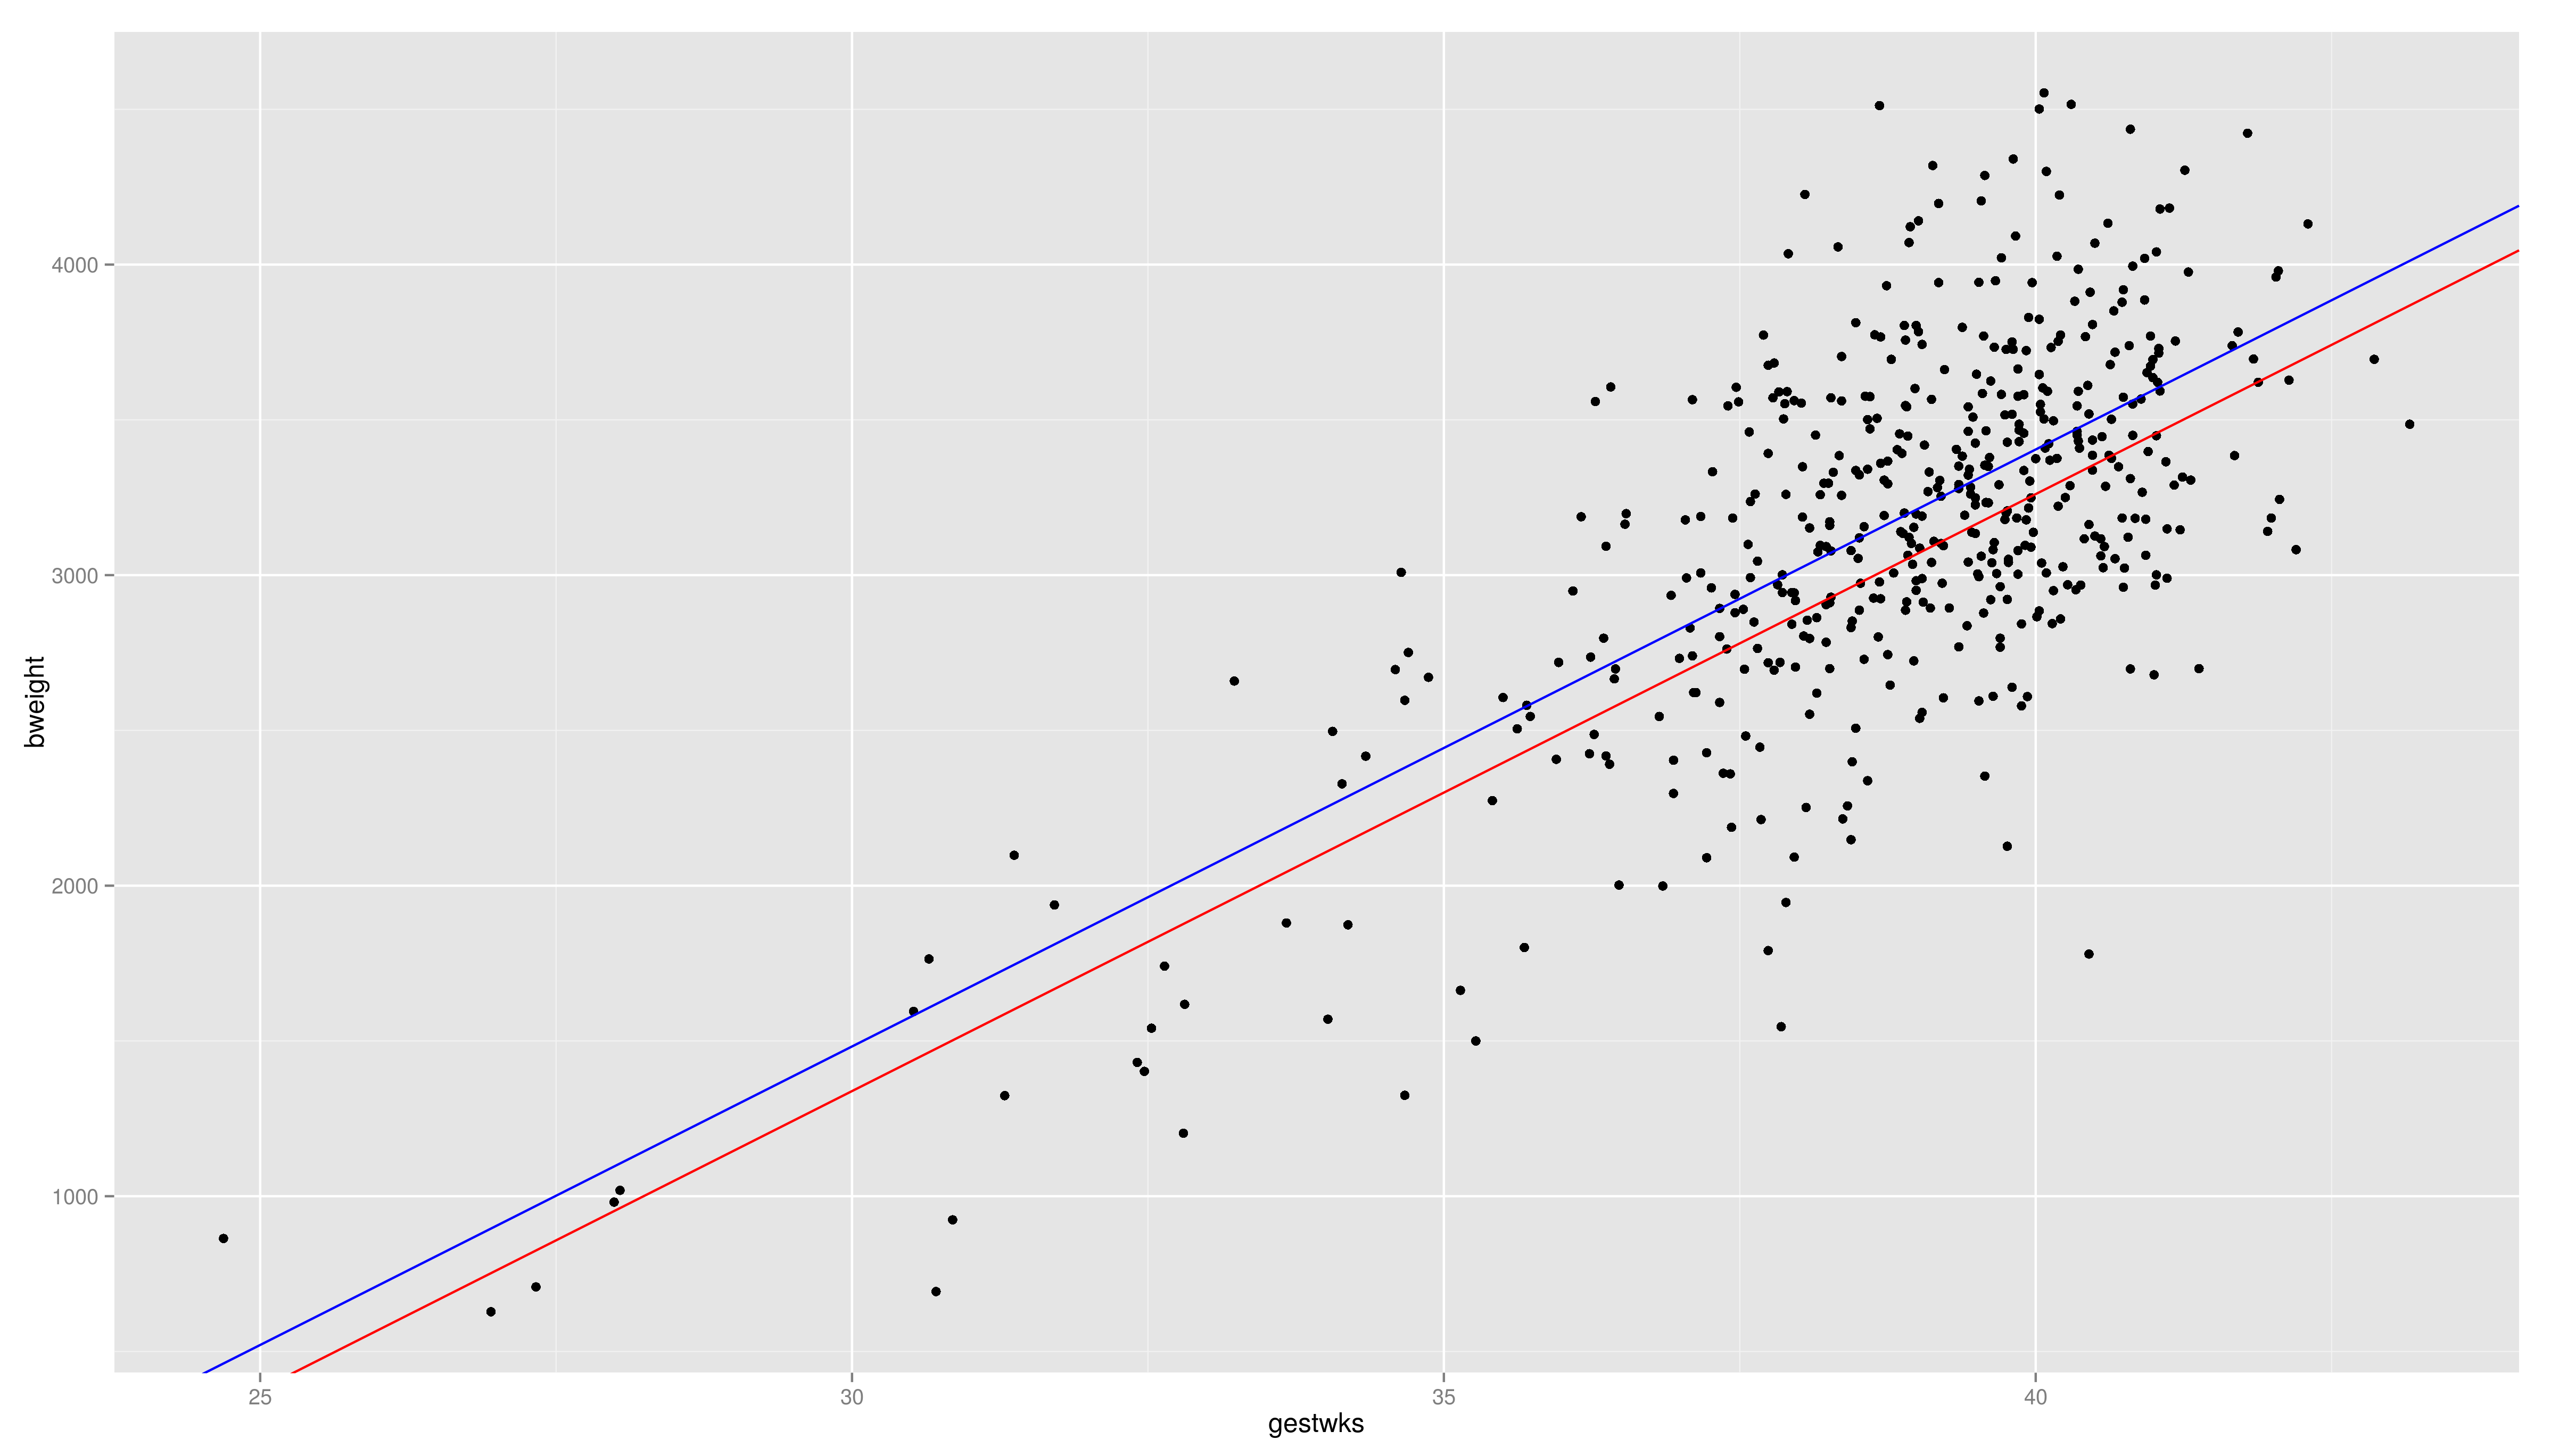
\includegraphics[height=7cm]{model2.png}

The effect of \texttt{gestwks} is the slope of the lines A and B (assumed to be the same). The effect of \texttt{hyp} ist the vertical distance between them.
\end{frame}


\begin{frame}{Our Example III}
  \begin{itemize}
  \item we add the interaction between \texttt{hyp} and \texttt{gestwks}
  \item so we estimate two intercepts and two slopes, one of each for each level of \texttt{hyp} 
  \end{itemize}
\end{frame}

\begin{frame}[fragile]{Our Example III}\scriptsize
\begin{semiverbatim}
> m <- lm(bweight ~ hyp * gestwks, data=births)
> summary(m)

Call:
lm(formula = bweight ~ hyp * gestwks, data = births)

Residuals:
     Min       1Q   Median       3Q      Max 
-1698.36  -291.13    -5.14   284.48  1359.16 

Coefficients:
                 Estimate Std. Error t value Pr(>|t|)    
(Intercept)      -3960.82     406.76  -9.738   <2e-16 ***
hyphyper         -1332.66     769.60  -1.732    0.084 .  
gestwks            183.91      10.43  17.626   <2e-16 ***
hyphyper:gestwks    31.39      20.26   1.549    0.122    
---
Signif. codes:  0 ‘***’ 0.001 ‘**’ 0.01 ‘*’ 0.05 ‘.’ 0.1 ‘ ’ 1

Residual standard error: 446.8 on 486 degrees of freedom
  (10 observations deleted due to missingness)
Multiple R-squared:  0.5156,	Adjusted R-squared:  0.5126 
F-statistic: 172.4 on 3 and 486 DF,  p-value: < 2.2e-16
\end{semiverbatim}
\end{frame}

\begin{frame}[fragile]{Our Example III}\scriptsize
\begin{semiverbatim}
> coef(m)
     (Intercept)         hyphyper          gestwks hyphyper:gestwks 
      -3960.8157       -1332.6563         183.9105          31.3851 
> ggplot(births, aes(x = gestwks,y = bweight)) +
+     geom_point() +
+     geom_abline(intercept = coef(m)[1],
+                 slope = coef(m)[3],colour="blue") +
+     geom_abline(intercept = coef(m)[1] + coef(m)[2],
+                 slope = coef(m)[3] + coef(m)[4],colour="red")
\end{semiverbatim}
\end{frame}


\begin{frame}[shrink=5]\frametitle{Our Example III - visualization}
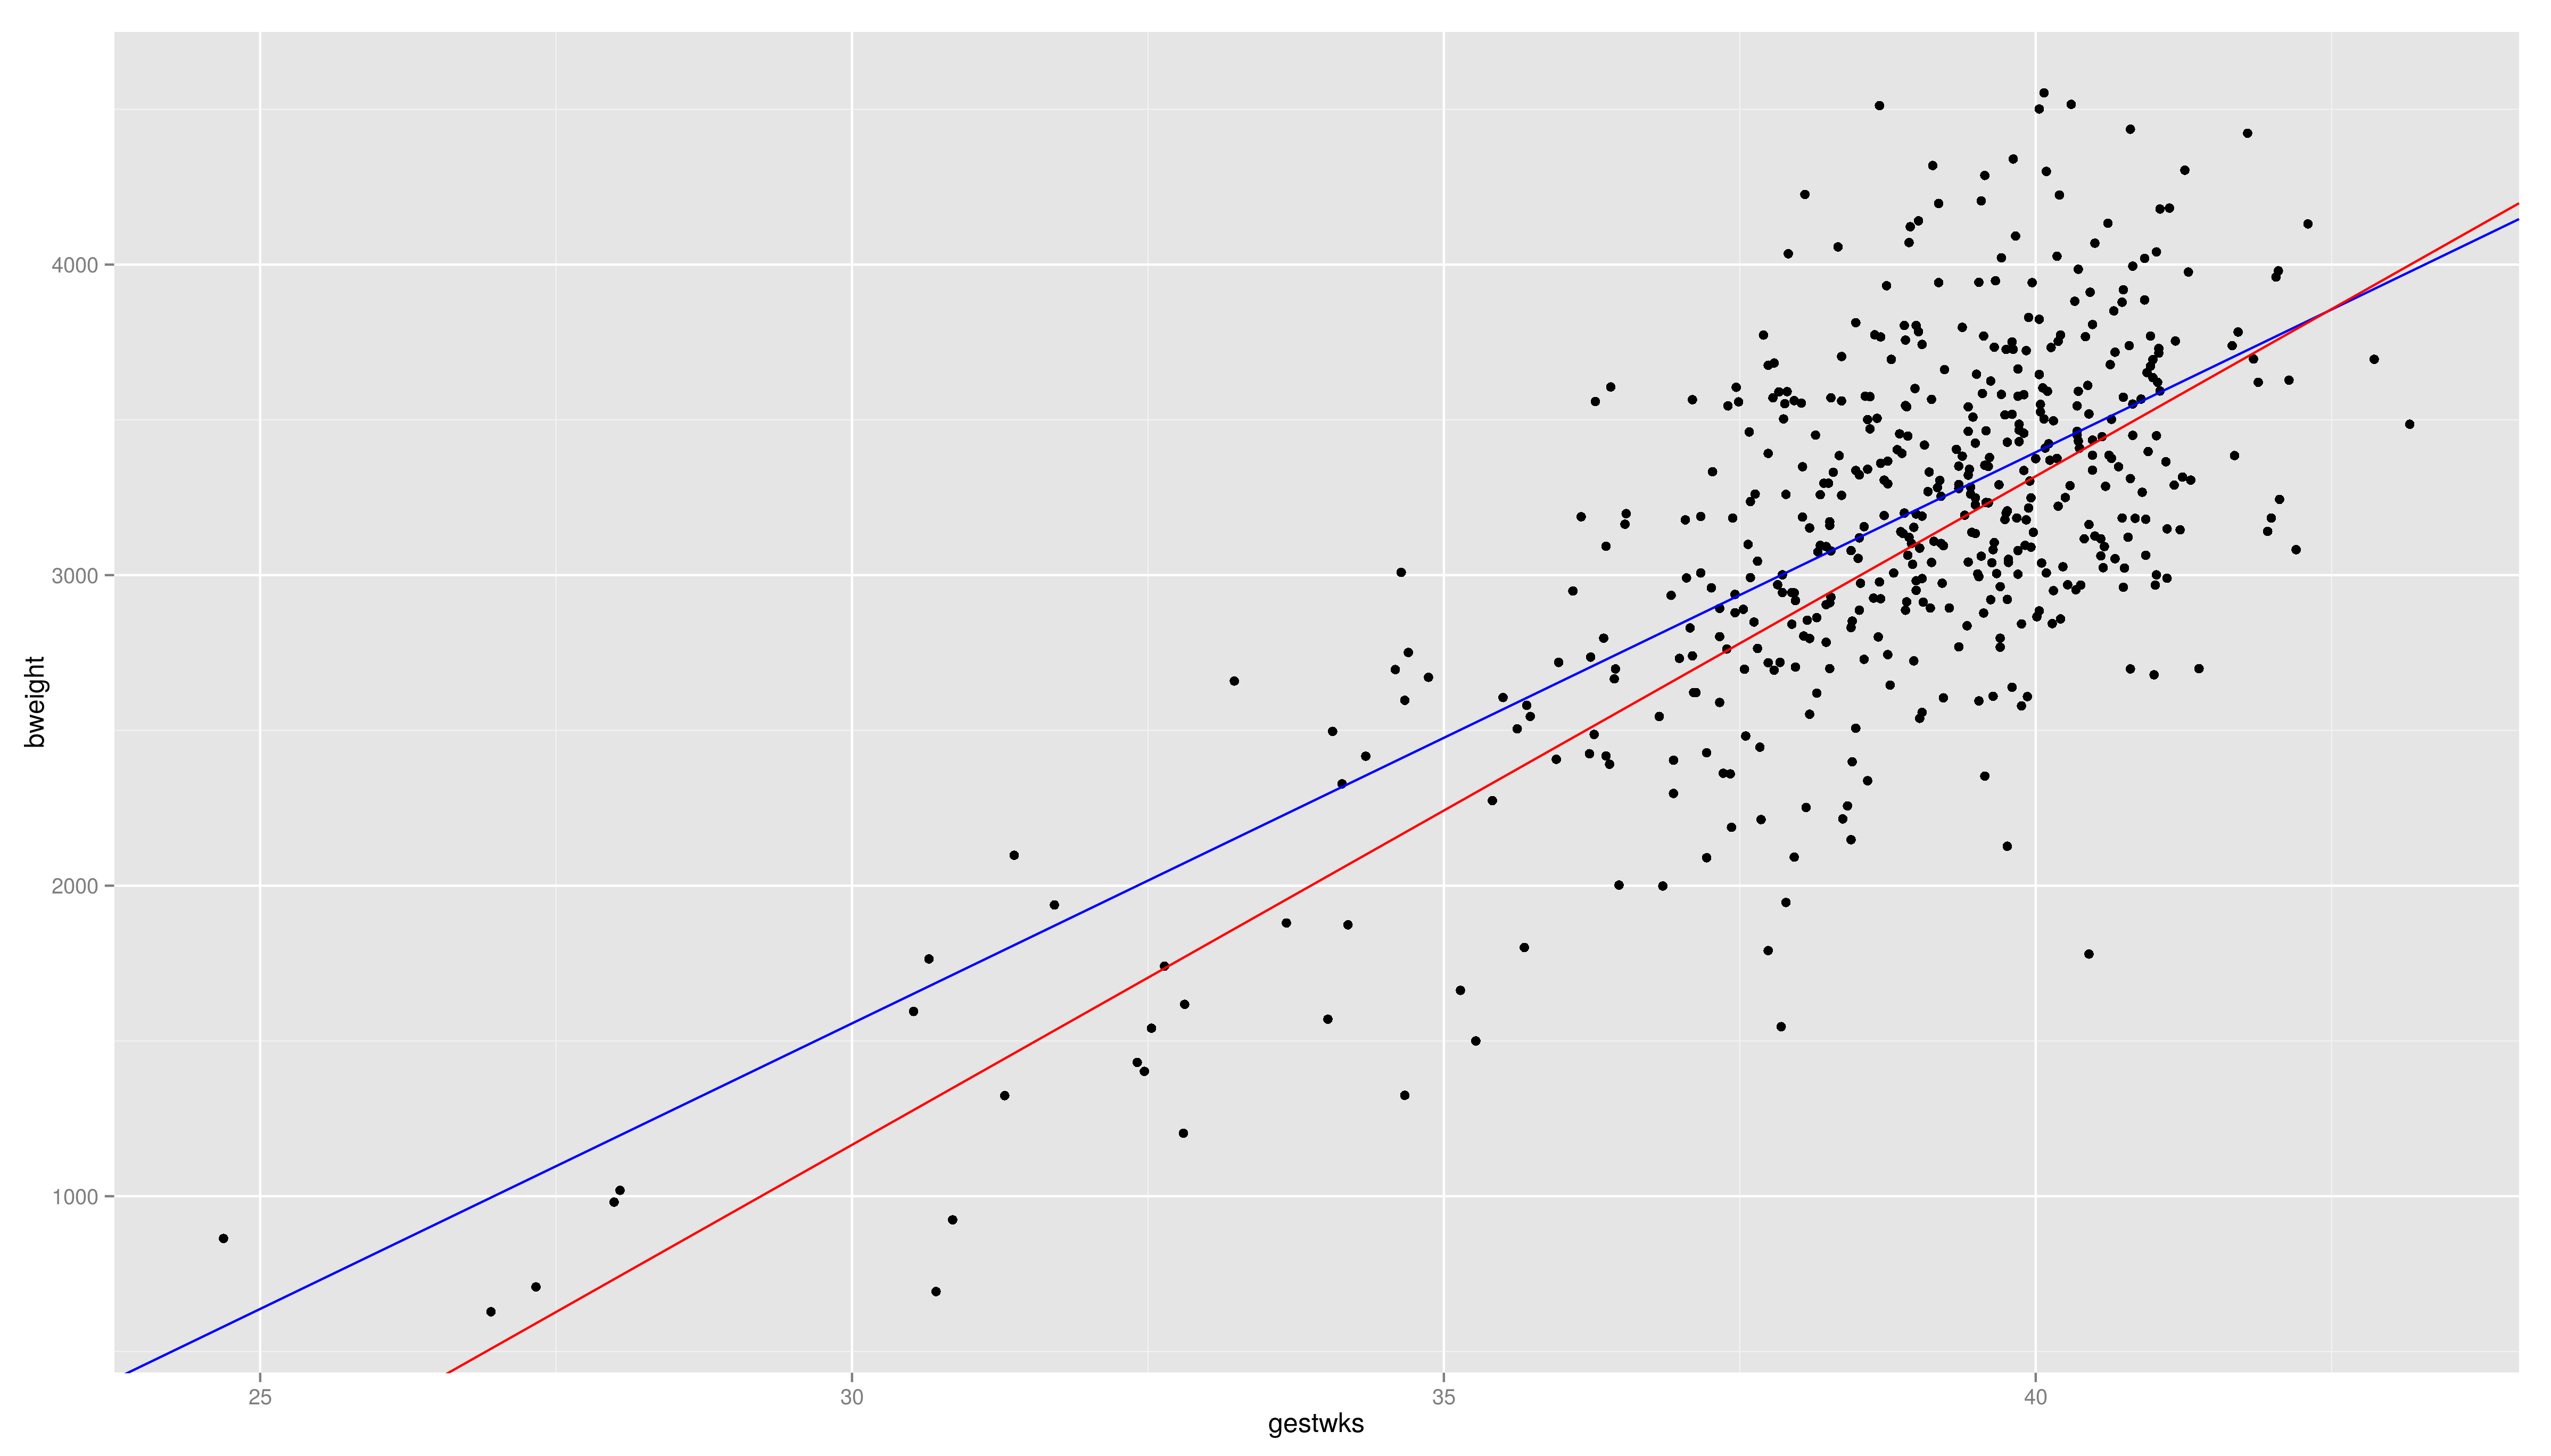
\includegraphics[height=7cm]{model3.png}

The effect of \texttt{gestwks} differs between groups. 
\end{frame}

\begin{frame}[fragile]{Our Example III}
  \begin{itemize}
  \item because of the difficulty to explain the coefficients we first center the variable \texttt{gestwks}
  \end{itemize}\scriptsize
\begin{verbatim}
> births$gwsc <- births$gestwks-40
> m <- lm(bweight ~ hyp * gwsc, data=births)
> coef(m)
  (Intercept)      hyphyper          gwsc hyphyper:gwsc 
   3395.60329     -77.25215     183.91048      31.38510 
\end{verbatim}
\end{frame}

\section{Exercises}

\begin{frame}[allowframebreaks]{Exercises}
  \begin{enumerate}
  \item  For the Cars93 (MASS) data set, answer the following:
    \begin{enumerate}
    \item For MPG. highway modeled by Horsepower, find the simple regression
coefficients. What is the predicted mileage for a car with 225 horsepower?
    \item Fit the linear model with MPG. highway modeled by Weight. Find the predicted highway mileage of a 6,400 pound HUMMER H2 and a 2,524 pound MINI Cooper.
    \item Fit the linear model Max .Price modeled by Min .Price. Why might you expect the slope to be around 1 ?
    \end{enumerate}
    Can you think of any other linear relationships among the variables?
  \item  For the data set MLBattend (UsingR) concerning major league baseball
attendance, fit a linear model of attendance modeled by wins. What is the predicted increase in attendance if a team that won 80 games last year wins 90 this year?
  \item  People often predict children’s future height by using their 2-year-old height. A common rule is to double the height. Table 10.2 contains data for eight people’s heights as 2-year-olds and as adults. Using the data, what is the predicted adult height for a 2-year-old who is 33 inches tall?

    \begin{tabular}{l c c c c c c c c}
      \hline
      Age 2 (inch) & 39 & 30 & 32 & 34 & 35 & 36 & 36 & 30 \\
      \hline
      Adult (in.) & 71 & 63 & 63 & 67 & 68 & 68 & 70 & 64 \\
      \hline
    \end{tabular}
  \item With the \texttt{rmr} (ISwR) data set, plot metabolic rate versus body weight. Fit a linear regression model to the relation. According to the fitted model, what is the predicted metabolic rate for a body weight of 70 kg? Give a
95\% confidence interval for the slope of the line.
  \item In the \textt{juul} (ISwR) data set, fit a linear regression model for the square root of the IGF-I concentration versus age to the group of subjects over 25 years old.
  \item In the \texttt{malaria} data set, analyze the log-transformed antibody level
versus age. Make a plot of the relation. Do you notice anything peculiar?
  \end{enumerate}
\end{frame}



\end{document}
